\section{Tidsplan}
Tidsplan for P1

Uge 41 8/10 – 12/10
Mandag den 8. Oktober                            Gruppedannelse og valg af emne.
Onsdag den 10. Oktober                          Indholdsfortegnelse skal laves færdig og sendes til vejleder.
Uge 42 15/10 - 19/10
 
Uge 43 22/10 – 26/10
Tirsdag den 23. Oktober                          Første deldeadline
Katrine står for initierende problem og afsnittet ”Hvad er komprimering.
Olav står for SMS teknologi – teori
Anders står for Algoritmer – forskellige metoder
Frederik står for Problemdokumentation
Jannek står for Målgruppe og det derunder
Kevin står for allerede eksisterende løsninger
Rikke står for tidsplanen
 
Uge 44 29/10 – 2/11
Mandag den 29. Oktober                         Anden deldeadline
                                                                 Katrine står for løsningsforslag
                                                                 Frederik står for afgrænsning
                                                                              	
Uge 45 5/11 – 9/11
Fredag den 9. November                         Møde kl 13.00 med bi-vejleder Amanda
Uge 46 12/11 – 16/11
Mandag den 12. November                      Udarbejde omkring 10 sider og fremlæggelse til statusseminar.
Tirsdag den 13. November                       Færdiggøre arbejde til statusseminar
Onsdag den 14. November                      Statusseminar begynder. 
Opponentgruppes fremlæggelse kl 8.00. 
Vores fremlæggelse kl 9.00

Uge 47 19/11 – 23/11
Mandag den 19. November                      Se på ”kritik” og råd fra statusseminar og ret hvor der skal rettes.
Tirsdag den 20. November                      Ret mangler i analyse del
Fredag den 23. November                       Påbegyndelse af løsning.
Uge 48 26/11 – 30/11
	Program til samling af sms beskeder. 
Udarbejdelse af afsnittet Løsninger.

Mandag den 26. November-                     Skrivning af program. 
Udarbejdelser af afsnit om programmet. 
Udarbejdelse af statisk bit-træ

Fredag den 30. November	Skrivning af program løsning. 
Udarbejdelser af afsnit om programmet.
Uge 49 3/12 – 7/12
Mandag den 3. December	Skrivning af program løsning. 
Skriv i rapporten om programmet.
Uge 50 10/12 – 14/12
	Færdiggørelse af programmet.
Færdiggørelse af afsnit Løsning.
Færdiggørelse af afsnit Konklusion.
Uge 51 17/12 – 21/12
Mandag den 17. December                     Korrekturlæsning.

Tirsdag den 18. December                     Sidste rettelser og gennemlæsning

Onsdag den 19. December                    P1 rapport afleveres senest kl. 12.00
	Udarbejdelse af procesanalyse.

Torsdag den 20. December	Udarbejdelse af procesanalyse.

Fredag den 21. December                    Aflevering af procesanalyse senest kl 9.00


\section{Arbejdsintensitet på GitHub}
\label{bilag2}
\begin{figure}[H]
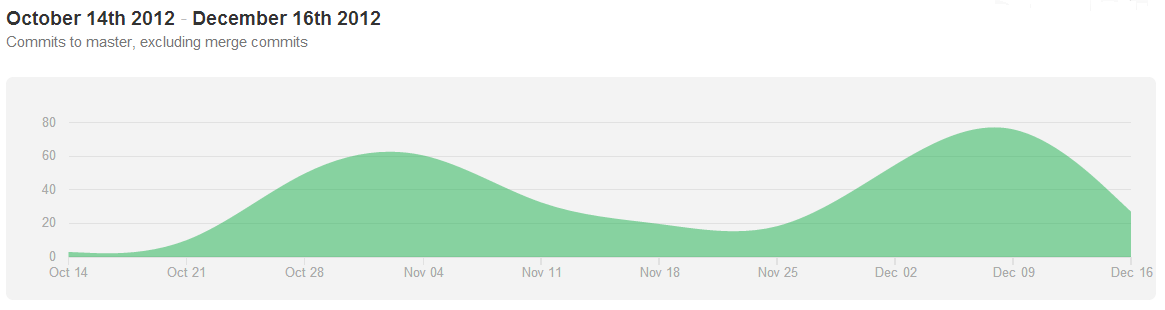
\includegraphics[width=\textwidth]{Indhold/arbejdsintensitet.png}
\caption {Billedet viser hvor ofte vi har "commitet" nye filer eller nyt arbejde til vores fælles mappe.}
\label {arbejde}
\end{figure}
